Предложенный алгоритм тестируется с помощью численного моделирования для функции логистической регрессии и 
сравнивается с классическими подходами.
Исходный код на языке Python доступен в открытом репозитории диссертации\footnote{\url{https://github.com/NMashalov/EducationGenerativeModelApplication}}.

Основным критерием для анализа является соотношение изменения параметра сложности задачи $\Delta d$ к параметру роста ${\beta}$.
Таким образом, были исследованы две ключевые краевые постановки: \begin{enumerate}
    \item малые изменения  $\Delta d / \beta \approx 0$;
    \item значительные изменения $\Delta d / \beta \approx 1$.
\end{enumerate}
В каждом эксперименте сравнивалась эффективность предложенного метода с эффективностью классического алгоритма Роббинса-Монро и его аналога с 
фиксированным коэффициентом $\lambda$ \cite{yazidi2020balanced}. Дополнительно изучено влияние модификации по методу Поляка скользящим средним. 

Гладкие графики траекторий получены путем визуализации среднего и перцентилей распределения. Для их численного расчета используется метод бутстрэп \cite{efron1994introduction}. 
Эксперимент проводился $B >> 1$ раз, после чего путем расчета распределения определялась статистика.   

В разделе приведены основные графики. Полный набор параметров доступен в приложении к работе. Отметим, что при анализе сходимости число шагов $N$ определяется
 аналогично правилу предела. $N$ считается шагом достижения сходимости, если все последующие точки не выходят за границу $\epsilon$.  Значение $\epsilon$ 
 выбирается индивидуально из соображений статистической значимости результата. 

\subsubsection{Случай $\Delta d / \beta \approx 1$ }
Эксперимент проводился для $s(d) = \frac{1}{1+\exp(-5(d-0.6)} $ c начальной сложностью $d_0 =0.2$ и целевым параметром $s^* =0.4$

Отметим также чувствительность алгоритма Роббинса-Монро к параметру шага \ref{exp1:classic}: 
\begin{figure}[h]
    \centering
    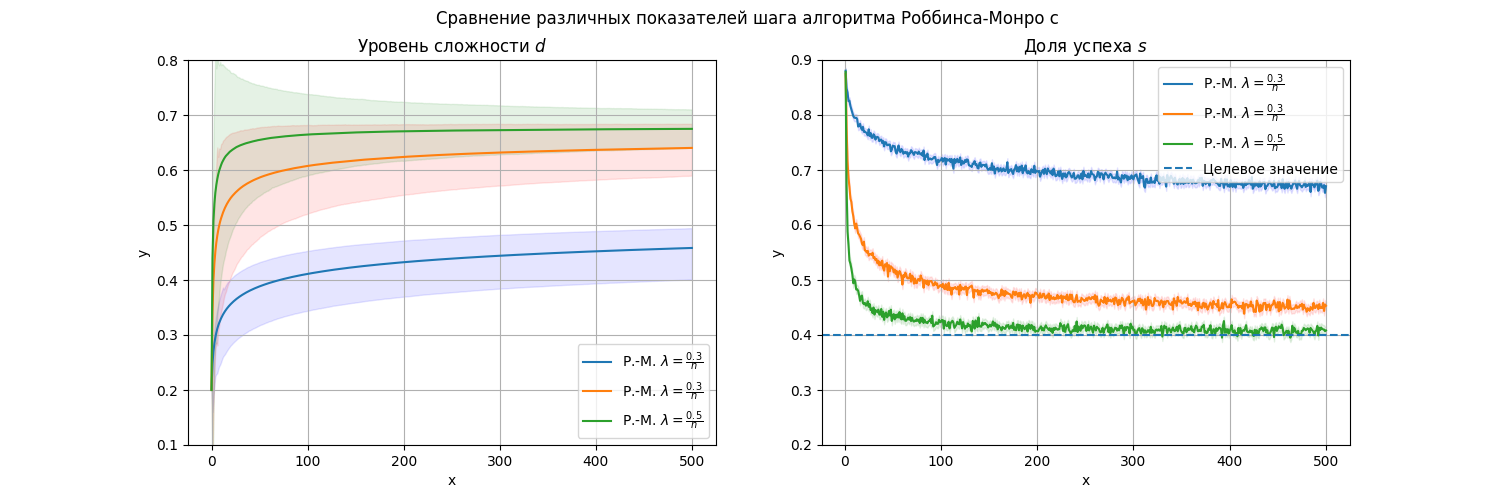
\includegraphics[width=1.0\textwidth]{assets/work/rating/1/sensitivity.png}
    \caption{Чувствительность классического алгоритма Роббинса-Монро к параметру $\lambda$}
    \label{exp1:classic}
\end{figure}
\begin{table}
    \centering
    \begin{tabular}{ ||c | c|| }
        \hline 
          \text{Алгоритм} &  \text{Число шагов}\\
        \hline 
         \text{Постоянный} $\lambda_n = 0.01$ & $400  \pm 20$ \\  
         \text{Алгоритм Р-М} $\lambda_n = 0.1$ & \text{Не сошелся} \\
         \text{Алгоритм Р-М} $\lambda_n = 0.5$ & $250 \pm 30$ \\
         \text{Адаптированный алгоритм Р-М} & $200 \pm 35 $   \\
         \hline
    \end{tabular}        
    \caption{Сравнение числа шагов сходимости в постановке $\Delta d / \beta \approx 1$}
    \label{exp1:table}
\end{table}
\subsubsection{Случай $\Delta d / \beta \approx 0$ }
Эксперимент проводился для $s(d) = \frac{1}{4(d-0.6)}$ c начальной сложностью $d_0 =0.2$ и целевым параметром $s=0.8$. 
Число раундов было выбрано минимальным для\footnote{Для наглядности в таблице классический алгоритм Роббинса-Монро 
представлен аббревиатурой "Р-М" с указанием параметра шага.}

\begin{figure}[h]
    \centering
    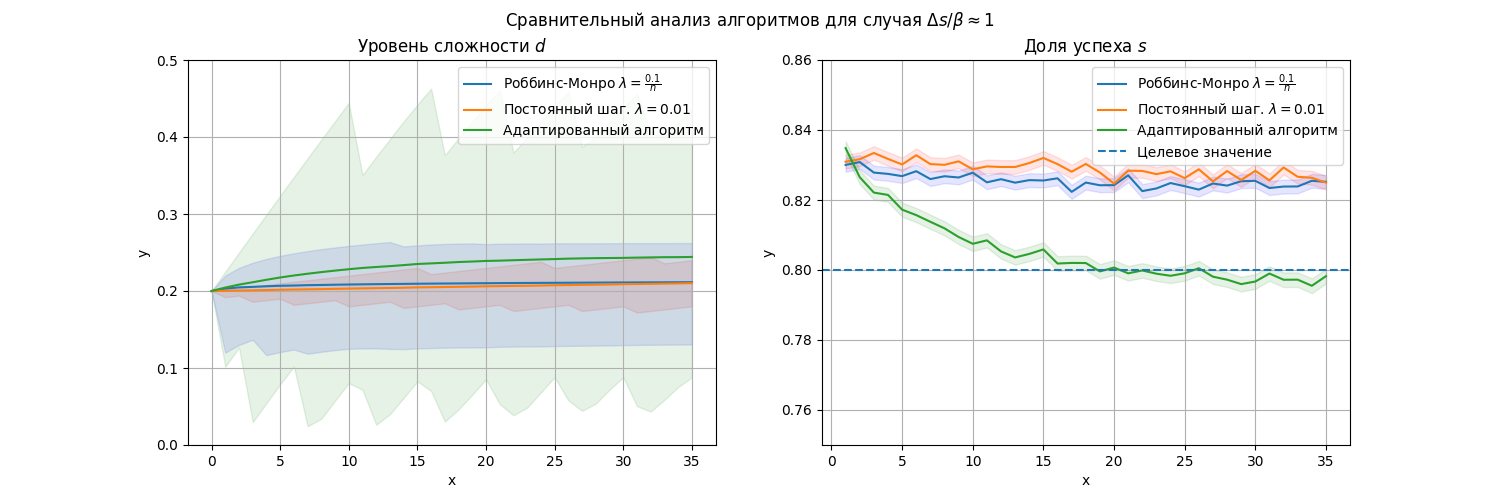
\includegraphics[width=1.0\textwidth]{assets/work/rating/2/comparison_analysis.png}
    \caption{Предложенный алгоритм имеет высокую скорость реакции $d$}
    \label{exp2:сomparison}
\end{figure}

\begin{table}
    \centering
    \begin{tabular}{ ||c | c|| }
        \hline 
        \text{Название алгоритма} &  \text{Число шагов}\\
        \hline 
        \text{Постоянный} $\lambda_n = 0.01$ & $400  \pm 20$ \\  
        \text{Алгоритм Р-М} $\lambda_n = 0.1$ & \text{Не сошелся} \\
        \text{Алгоритм Р-М} $\lambda_n = 0.5$ & $250 \pm 30$ \\
        \text{Адаптированный алгоритм  Р-М} & $200 \pm 35 $   \\
        \hline
    \end{tabular}
    \caption{Сравнение числа шагов сходимости в постановке $\Delta d / \beta \approx 0$.}
    \label{exp2:table}
\end{table}

\subsubsection{Случай значительного отличия априорных представлений о наклоне кривой от действительного}
Рассмотрен случай, в котором априорное значение $\beta$ значительно отличается от действительного значения $\beta^*$.
\begin{figure}[h]
    \centering
    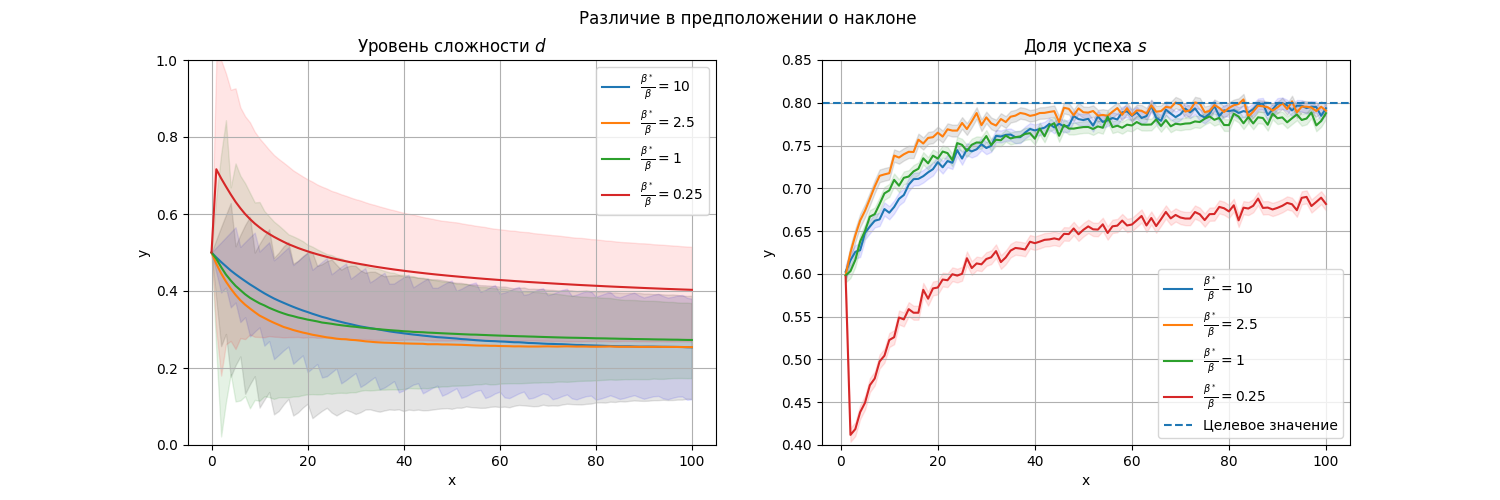
\includegraphics[width=0.9\textwidth]{assets/work/rating/3/slop_affect.png}
    \caption{Значительные различия в предположениях о наклоне логистической регрессии приводят к снижению эффективности алгоритма}
    \label{exp3:lose_effictivness}
\end{figure}
\begin{table}
    \centering
    \begin{tabular}{ ||c | c|| }
        \hline 
        \text{Название алгоритма} &  \text{Число шагов}\\
        \hline 
        \text{Адаптированный алгоритм Р-М} $\frac{\beta^*}{\beta}=10$  & $400  \pm 20$ \\  
        \text{Адаптированный алгоритм Р-М} $\frac{\beta^*}{\beta}=2.5$ & \text{Не сошелся} \\
        \text{Адаптированный алгоритм Р-М} $\frac{\beta^*}{\beta}=1$ & $250 \pm 30$ \\
        \text{Адаптированный алгоритм Р-М} $\frac{\beta^*}{\beta}=0.25$ & $200 \pm 35 $   \\
        \hline
    \end{tabular}
    \caption{Сравнение числа шагов сходимости в постановке различающихся априорных представлений о наклоне кривой
     от действительных}
    \label{exp3:table}
\end{table}
\subsubsection{Модификация скользящим средним}
Численно исследуем применимость метода скользящего среднего к предложенному алгоритму и алгоритму с постоянным шагом. 
\begin{figure}[h]
    \centering
    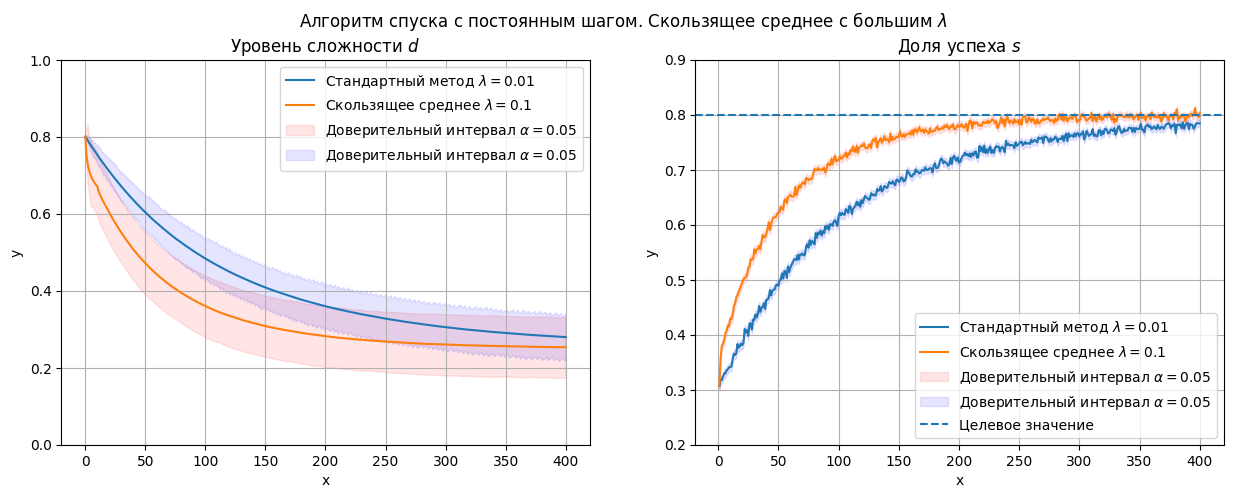
\includegraphics[width=0.9\textwidth]{assets/work/rating/4/lambda_0.01_0.1.png}
    \caption{Метод скользящего среднего позволяет использовать больший шага, не теряя устойчивость метода}
    \label{exp4:better_stability}
\end{figure}
\begin{figure}[h]
    \centering
    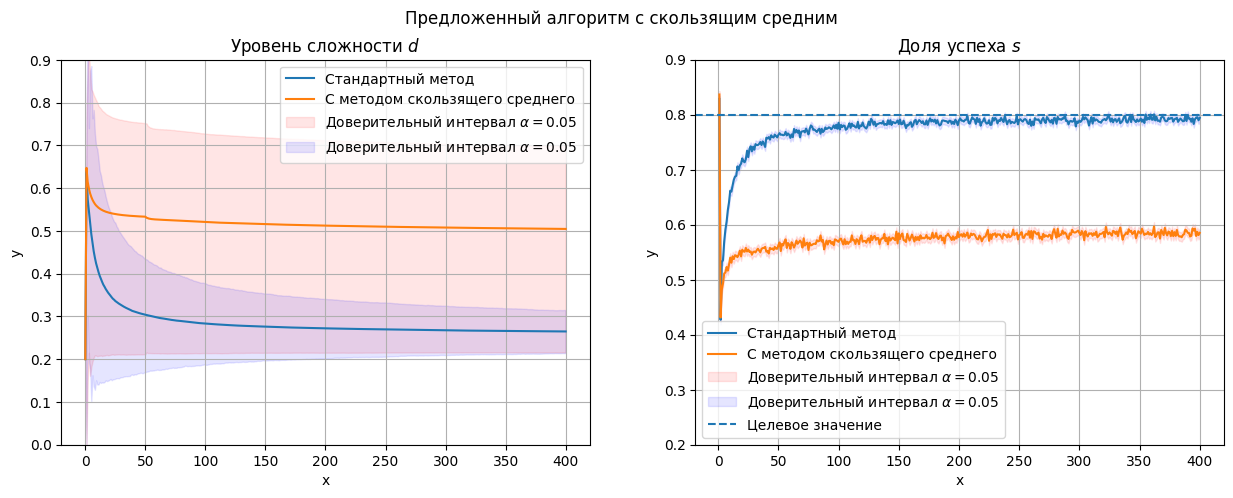
\includegraphics[width=0.9\textwidth]{assets/work/rating/4/adaptive.png}
    \caption{Метод скользящего среднего неприменим к предложенному алгоритму}
    \label{exp4:not_applied}
\end{figure}
\begin{table}
    \centering
    \begin{tabular}{ ||c | c|| }
        \hline
        \text{Название алгоритма} &  \text{Число шагов}\\
        \hline 
        \text{Алгоритм Р-М со скользящим средним $\lambda=0.01$} & \text{Не сошелся} \\
        \text{Алгоритм Р-М со скользящим средним $\lambda=0.1$} & $250\pm 40$  \\
        \text{Адаптированный алгоритм  Р-М со скользящим средним } & \text{Не сошелся}\\
        \hline 
    \end{tabular}
    \caption{Сравнение числа шагов с применением метода скользящего среднего}
    \label{exp4:table}
\end{table}

Расходимость предложенного метода связана с нарушениями условий на инфинизетемальность шага \ref{polyak_assumptions}.

Таким образом, метод скользящего среднего:
\begin{enumerate}
    \item позволяет использовать увеличенный шаг для обеспечения большей скорости сходимости;
    \item не применим к предложенному алгоритму.
\end{enumerate}

Полный набор задач моделирования приведен в приложении к работе \ref{numeric_modeling}.